\begin{geoitem}{Instrument Tube Pin Geometry}{fig_instr_pin}\centering
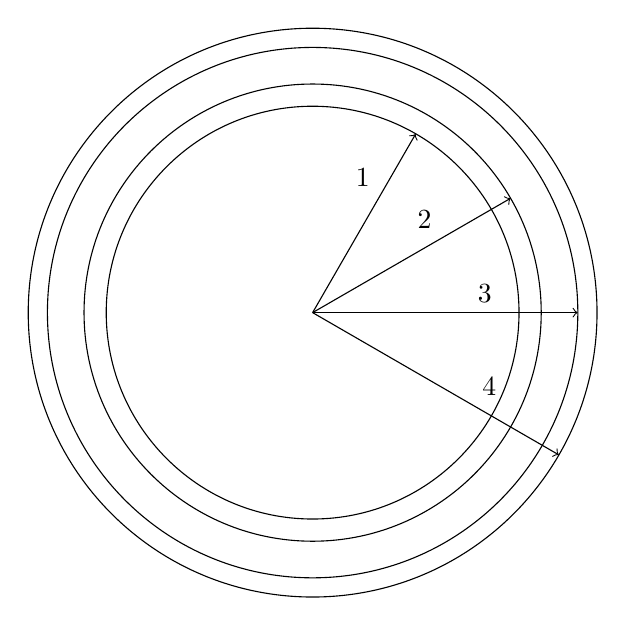
\begin{tikzpicture}[scale=6,auto]
        \draw (0,0) circle (0.43688);
      \draw[->] (0,0) -- node[pos=0.65] {1} (0.218,0.378);
      \draw (0,0) circle (0.48387);
      \draw[->] (0,0) -- node[pos=0.65] {2} (0.419,0.242);
      \draw (0,0) circle (0.56134);
      \draw[->] (0,0) -- node[pos=0.65] {3} (0.561,0.0);
      \draw (0,0) circle (0.60198);
      \draw[->] (0,0) -- node[pos=0.65] {4} (0.521,-0.301);

      \end{tikzpicture}
      \begin{tikzpicture}
       \matrix [matrix of nodes]
      {
          Arrow & Radius (cm) & Material & \numrefheader \\
        1 & 0.43688 & \node[hyperlink node=mat_air]{Air}; & \ref{num:ITthimIR}\\ 
        2 & 0.48387 & \node[hyperlink node=mat_zirc]{Zircaloy}; & \ref{num:ITthimOR}\\ 
        3 & 0.56134 & \node[hyperlink node=mat_water]{Water}; & \ref{num:GTIRrad}\\ 
        4 & 0.60198 & \node[hyperlink node=mat_zirc]{Zircaloy}; & \ref{num:GTORrad}\\ 
      };
\end{tikzpicture}
\\ \raggedright The thimble radii were chosen to be equivalent to the outer
thimble radii of control rods and burnable absorber rods by assumption. Note
that not all instrument tube positions contain the thimble defined by the first
2 radii in the diagram above, as discussed in Section \ref{sec:coreinstrpos}.
This pincell does not change at the dashpot.
\end{geoitem}

\begin{geoitem}{Bare Instrument Thimble Pin Geometry}{fig_instr_pin_bare}\centering
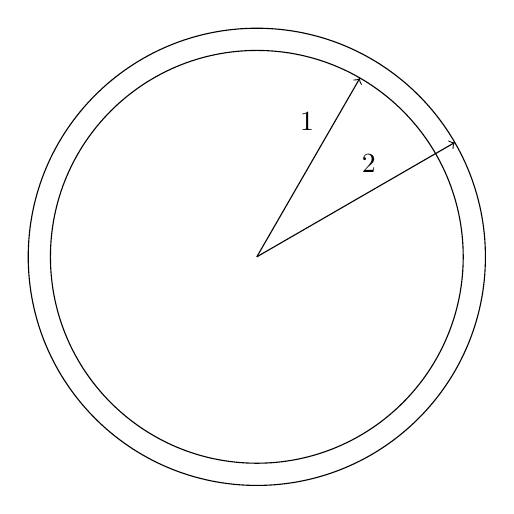
\begin{tikzpicture}[scale=6,auto]
        \draw (0,0) circle (0.43688);
      \draw[->] (0,0) -- node[pos=0.65] {1} (0.218,0.378);
      \draw (0,0) circle (0.48387);
      \draw[->] (0,0) -- node[pos=0.65] {2} (0.419,0.242);

      \end{tikzpicture}
      \begin{tikzpicture}
       \matrix [matrix of nodes]
      {
          Arrow & Radius (cm) & Material & \numrefheader \\
        1 & 0.43688 & \node[hyperlink node=mat_air]{Air}; & \ref{num:ITthimIR}\\ 
        2 & 0.48387 & \node[hyperlink node=mat_zirc]{Zircaloy}; & \ref{num:ITthimOR}\\ 
      };
\end{tikzpicture}
\\ \raggedright The bare instrument thimble for regions below the instrument tube.
\end{geoitem}
